% command to make sure colorboxes don't create whitespace between code lines
\fboxsep=.6pt

% default settings for listings (MicroPython on the Raspberry Pi Pico)
\lstset{style=python, basicstyle=\ttfamily\footnotesize}

\title[Robotik]{Analoge Signale \& PWM}
\subtitle{Vom Potentiometer zur realistischen LED-Kerze}

% \author[Graf, Thomas]
% {}

\institute[KLW]
{
	Kantonsschule Im Lee
}

\date[\today]

\logo{\includegraphics[width=2cm]{Logos/FreeFlower.pdf}}

\titlegraphic{\vspace{-.7cm}\includegraphics[width=\textwidth]{"Grundlagen_Info/06_Datenbanken/Figures/title-emojis"}}

\frame{\titlepage}

\begin{frame}{Auftrag und Lernziele}
	Am Ende der Doppellektion können Sie \ldots
	\begin{itemize}[<+->]
		\item erklären, wie ein ADC eine Spannung in eine Zahl übersetzt;
		\item erklären, wie PWM mit digitalen Pulsen eine LED dimmt;
		\item eine LED mit richtig gepoltem Anschluss und Vorwiderstand aufbauen;
		\item den Algorithmus aus dem Video lesen und auf MicroPython übertragen;
		\item eine LED-Kerze mit mehreren, unabhängig flackernden LEDs bauen.
	\end{itemize}
\end{frame}

\begin{frame}{Motivation: Die Welt ist nicht nur 0 oder 1}
	\begin{itemize}[<+->]
		\item Ein digitaler Pin kennt zwei Zustände: \textbf{LOW} und \textbf{HIGH}.
		\item Viele Grössen unserer Umwelt ändern sich jedoch kontinuierlich:
		\begin{itemize}
			\item Lichtstärke, Temperatur, Lautstärke, Position eines Drehknopfs.
		\end{itemize}
		\item Zwei Übersetzer verbinden beide Welten:
		\begin{itemize}
			\item \textbf{ADC (Analog-to-Digital Converter, Analog-Digital-Wandler):}
			analoge Spannung $\rightarrow$ digitale Zahl
			\item \textbf{PWM (Pulse Width Modulation, Pulsweitenmodulation):}
			digitale Pulse $\rightarrow$ wahrgenommene Helligkeit
		\end{itemize}
	\end{itemize}
\end{frame}

\begin{frame}{Analog-Digital-Wandler (ADC)}
	\begin{itemize}[<+->]
		\item Der ADC vergleicht die Eingangsspannung mit einer Referenzspannung.
		\item Ein idealer ADC mit $n$ Bit liefert Werte von $0$ bis $2^n-1$.
		\item Beispiel mit $n=10$ und $U_\mathrm{ref}=\qty{3.3}{\volt}$:
		\begin{itemize}
			\item $\qty{0}{\volt}\rightarrow 0$
			\item $\qty{3.3}{\volt}\rightarrow 1023$
		\end{itemize}
	\end{itemize}
	\[
		U_\mathrm{in}\approx\frac{\text{Messwert}}{2^n-1}\,U_\mathrm{ref}
	\]
\end{frame}

\begin{frame}{Eingabe messen}
	\begin{myexercise}
		Ein \qty{10}{\bit}-ADC liefert den Messwert $512$. Die Referenzspannung beträgt
		$U_\mathrm{ref}=\qty{3.3}{\volt}$. Welche Spannung liegt ungefähr am Pin an?
	\end{myexercise}
\end{frame}

\begin{frame}{Eingabe messen -- Lösung}
	\begin{myanswer}
		\[
			U_\mathrm{in}=\frac{512}{1023}\cdot\qty{3.3}{\volt}
			\approx\qty{1.65}{\volt}
		\]
		Der kleine Unterschied zwischen $1023$ und $1024$ ist hier praktisch nicht sichtbar:
		$1023$ ist der grösste darstellbare Wert, $1024$ die Anzahl möglicher Werte.
	\end{myanswer}
\end{frame}

\begin{frame}{Das Potentiometer als Spannungsteiler}
	\begin{columns}[T]
		\begin{column}{0.55\textwidth}
			\begin{itemize}[<+->]
				\item Die beiden äusseren Pins kommen an \qty{3.3}{\volt} und GND.
				\item Der mittlere Pin (Schleifer) kommt an einen ADC-Pin.
				\item Beim Drehen ändert sich die Ausgangsspannung zwischen
				\qty{0}{\volt} und \qty{3.3}{\volt}.
				\item Die Reihenfolge der äusseren Pins bestimmt nur die Drehrichtung.
			\end{itemize}
		\end{column}
		\begin{column}{0.42\textwidth}
			\centering
			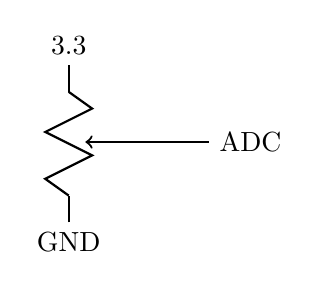
\begin{tikzpicture}[thick,scale=.85]
				\draw (0,0) node[below]{GND} -- (0,.4);
				\draw (0,.4) -- (-.35,.65) -- (.35,1.0) -- (-.35,1.35) -- (.35,1.7) -- (0,1.95);
				\draw (0,1.95) -- (0,2.35) node[above]{\qty{3.3}{\volt}};
				\draw[->] (1.5,1.2) -- (.25,1.2);
				\draw (1.5,1.2) -- (2.1,1.2) node[right]{ADC};
			\end{tikzpicture}
		\end{column}
	\end{columns}
\end{frame}

\begin{frame}{Ausgabe: Wie dimmen wir eine LED?}
	\begin{itemize}[<+->]
		\item Ein digitaler Pin liefert näherungsweise \qty{0}{\volt} oder \qty{3.3}{\volt}.
		\item Bei der \textbf{Pulsweitenmodulation (PWM)} wird sehr schnell ein- und ausgeschaltet.
		\item Bei einer PWM-Frequenz von z.\,B. \qty{1}{\kilo\hertz} dauert eine Periode
		$T=1/f=\qty{1}{\milli\second}$.
		\item Das Auge nimmt hauptsächlich die mittlere Helligkeit wahr.
	\end{itemize}
	\pause
	\[
		D=\frac{t_\mathrm{ein}}{T}
	\]
	\begin{itemize}[<+->]
		\item $D$: Tastgrad, also Anteil der Einschaltzeit an einer Periode
		\item $t_\mathrm{ein}$: Zeit, während der die LED innerhalb einer Periode eingeschaltet ist
		\item $T$: Dauer einer vollständigen Periode; es gilt $T=1/f$
	\end{itemize}
\end{frame}

\begin{frame}{PWM: Tastgrad statt echter Analogspannung}
	\begin{itemize}
		\item \qty{25}{\percent}: kurz an, lange aus $\rightarrow$ eher dunkel
		\item \qty{75}{\percent}: lange an, kurz aus $\rightarrow$ eher hell
	\end{itemize}
	\begin{center}
		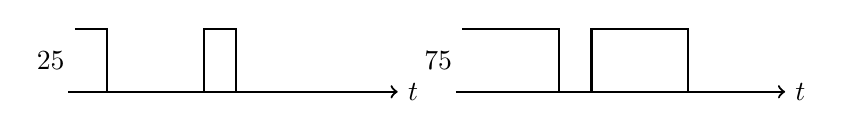
\begin{tikzpicture}[xscale=.82,yscale=.8,thick]
			\draw[->] (-.1,0) -- (5,0) node[right] {$t$};
			\draw (0,1) -- (.5,1) -- (.5,0) -- (2,0) -- (2,1) -- (2.5,1) -- (2.5,0) -- (4,0);
			\node[left] at (0,.5) {\qty{25}{\percent}};
			\begin{scope}[xshift=6cm]
				\draw[->] (-.1,0) -- (5,0) node[right] {$t$};
				\draw (0,1) -- (1.5,1) -- (1.5,0) -- (2,0) -- (2,1) -- (3.5,1) -- (3.5,0) -- (4,0);
				\node[left] at (0,.5) {\qty{75}{\percent}};
			\end{scope}
		\end{tikzpicture}
	\end{center}
	\pause
	\textbf{Wichtig:} Die LED erhält weiterhin volle Pulse; PWM senkt nicht einfach die Pinspannung.
\end{frame}

\begin{frame}{LED richtig und sicher anschliessen}
	\begin{columns}[T]
		\begin{column}{0.56\textwidth}
			\begin{itemize}[<+->]
				\item Langes Bein: Anode ($+$); kurzes Bein: Kathode ($-$).
				\item Die abgeflachte Gehäuseseite markiert meist die Kathode.
				\item \textbf{Jede LED braucht einen eigenen Vorwiderstand.}
				\item Beispiel für eine gelbe LED mit $U_F\approx\qty{2.0}{\volt}$ und
				$I\approx\qty{6}{\milli\ampere}$:
			\end{itemize}
			\[
				R=\frac{\qty{3.3}{\volt}-\qty{2.0}{\volt}}{\qty{6}{\milli\ampere}}
				\approx\qty{217}{\ohm}
			\]
			Ein Normwert von \qty{220}{\ohm} passt.
		\end{column}
		\begin{column}{0.40\textwidth}
			\centering
			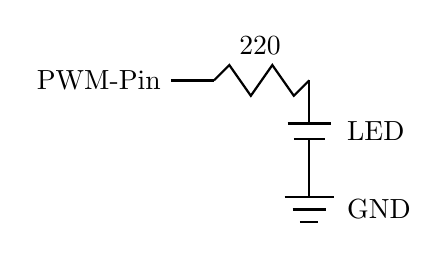
\begin{tikzpicture}[thick,scale=.78]
				\node[left] at (0,2.6) {PWM-Pin};
				\draw (0,2.6) -- (.7,2.6);
				\draw (.7,2.6) -- (.95,2.85) -- (1.3,2.35) -- (1.65,2.85) -- (2,2.35) -- (2.25,2.6);
				\node[above] at (1.45,2.85) {\qty{220}{\ohm}};
				\draw (2.25,2.6) -- (2.25,1.9);
				\draw (1.9,1.9) -- (2.6,1.9);
				\draw (2.0,1.65) -- (2.5,1.65);
				\draw (2.25,1.65) -- (2.25,.7);
				\draw (1.85,.7) -- (2.65,.7);
				\draw (1.98,.5) -- (2.52,.5);
				\draw (2.1,.3) -- (2.4,.3);
				\node[right] at (2.7,1.78) {LED};
				\node[right] at (2.7,.5) {GND};
			\end{tikzpicture}
		\end{column}
	\end{columns}
\end{frame}

\begin{frame}{Videoauftrag: Beobachten, dann erklären}
	\begin{columns}[T]
		\begin{column}{0.68\textwidth}
			\textbf{Video:} \href{https://www.youtube.com/watch?v=uX9YMCLgK9A}{Realistic Candle Light with LED Arduino PWM}
			\begin{enumerate}
				\item Wie viele LEDs und PWM-Pins werden verwendet?
				\item Welche Werte kann \lstinline|random(120)+135| erzeugen?
				\item Weshalb startet der Bereich nicht bei $0$?
				\item Weshalb erhält jede LED einen eigenen Zufallswert?
				\item Welche Pausenlängen erzeugt \lstinline|delay(random(100))|?
			\end{enumerate}
		\end{column}
		\begin{column}{0.28\textwidth}
			\centering
			\qrcode[height=2.6cm]{https://www.youtube.com/watch?v=uX9YMCLgK9A}

			\vspace{.3cm}
			\scriptsize Dauer: ca. \qty{5.2}{\minute}
		\end{column}
	\end{columns}
\end{frame}

\begin{frame}[fragile]{Den Arduino-Code aus dem Video lesen}
\begin{lstlisting}[language=C++]
void loop() {
  analogWrite(9,  random(120) + 135);
  analogWrite(10, random(120) + 135);
  analogWrite(11, random(120) + 135);
  delay(random(100));
}
\end{lstlisting}
	\begin{itemize}
		\item \lstinline|random(120)| liefert ganze Zahlen von $0$ bis $119$.
		\item Damit liegt der PWM-Wert zwischen $135$ und $254$ (von maximal $255$).
		\item Die LED erlischt nie ganz; drei unabhängige Werte erzeugen bewegtes Licht.
		\item Die Pause variiert zwischen \qty{0}{\milli\second} und \qty{99}{\milli\second}.
	\end{itemize}
\end{frame}

\begin{frame}{Vom Video zum Modell}
	Eine überzeugende Kerze kombiniert drei Ideen:
	\begin{enumerate}[<+->]
		\item \textbf{Warme Farben:} gelbe, orange und rote LEDs mischen ihr Licht.
		\item \textbf{Grundhelligkeit:} Die LEDs bleiben meistens deutlich sichtbar.
		\item \textbf{Unregelmässigkeit:} Helligkeit und Wartezeit ändern sich zufällig.
	\end{enumerate}
	\pause
	\begin{myexercise}
		Erklären Sie, was unrealistisch wirken würde, wenn alle drei LEDs stets denselben
		Zufallswert erhielten oder die Pause immer genau \qty{50}{\milli\second} dauerte.
	\end{myexercise}
\end{frame}

\begin{frame}{Material und Verdrahtung (Raspberry Pi Pico)}
	\begin{columns}[T]
		\begin{column}{0.48\textwidth}
			\textbf{Material}
			\begin{itemize}
				\item Raspberry Pi Pico mit MicroPython
				\item je eine rote, orange und gelbe LED
				\item drei Widerstände zu je \qty{220}{\ohm}
				\item Breadboard und Jumper-Kabel
				\item optional: \qty{10}{\kilo\ohm}-Potentiometer
				\item Diffusor aus Transparentpapier
			\end{itemize}
		\end{column}
		\begin{column}{0.48\textwidth}
			\textbf{Verbindungen}
			\begin{itemize}
				\item GP13 $\rightarrow$ \qty{220}{\ohm} $\rightarrow$ LED rot $\rightarrow$ GND
				\item GP14 $\rightarrow$ \qty{220}{\ohm} $\rightarrow$ LED orange $\rightarrow$ GND
				\item GP15 $\rightarrow$ \qty{220}{\ohm} $\rightarrow$ LED gelb $\rightarrow$ GND
				\item optionales Poti: \qty{3.3}{\volt}, GP26/ADC0, GND
			\end{itemize}
			\alert{Vor dem Umstecken: Stromversorgung trennen.}
		\end{column}
	\end{columns}
\end{frame}

\begin{frame}[fragile]{MicroPython: Version wie im Video}
\begin{lstlisting}[language=Python]
from machine import Pin, PWM
from random import randint
from time import sleep_ms

leds = []
for pin_number in (13, 14, 15):
    pin = Pin(pin_number)
    led = PWM(pin)
    led.freq(1000)                 # 1 kHz
    leds.append(led)

while True:
    for led in leds:
        value_8bit = randint(135, 254)
        led.duty_u16(value_8bit * 257)  # 8 Bit -> 16 Bit
    sleep_ms(randint(0, 99))
\end{lstlisting}
	\begin{itemize}
		\item \lstinline|duty_u16| erwartet eine \qty{16}{\bit}-Zahl. Der grösste mögliche Wert ist
		$2^{16}-1=\num{65535}$; er bedeutet \qty{100}{\percent} Tastgrad.
		\item Der Videocode verwendet \qty{8}{\bit}: $0$ bis $2^8-1=255$. Der Faktor
		$\num{257}$ bildet diesen Bereich exakt auf $0$ bis $\num{65535}$ ab, denn
		$255\cdot\num{257}=\num{65535}$.
	\end{itemize}
\end{frame}

\begin{frame}{Bauauftrag: LED-Kerze}
	\begin{enumerate}[<+->]
		\item Bauen Sie zuerst \textbf{eine} LED mit \qty{220}{\ohm} auf und testen Sie sie.
		\item Ergänzen Sie die beiden weiteren LEDs -- jede mit eigenem Widerstand.
		\item Übertragen und starten Sie das MicroPython-Programm.
		\item Prüfen Sie: Flackern alle LEDs unabhängig? Bleiben sie stets leicht an?
		\item Formen Sie einen Diffusor, ohne leitendes Material an die Kontakte zu bringen.
		\item Variieren Sie Wertebereich und Pause und dokumentieren Sie Ihre beste Einstellung.
	\end{enumerate}
\end{frame}

\begin{frame}{Fehlersuche: systematisch statt zufällig}
	\begin{tabularx}{\textwidth}{@{}lX@{}}
		\toprule
		\textbf{Beobachtung} & \textbf{Prüfen} \\
		\midrule
		LED bleibt dunkel & Polung, GND-Verbindung, Pin-Nummer, Widerstand und Programmstart \\
		LED leuchtet konstant & PWM-Objekt verwendet? Schleife aktiv? Richtiger GPIO? \\
		Alle LEDs flackern gleich & Wird für jede LED ein neuer Zufallswert erzeugt? \\
		Flackern wirkt hektisch & Untere Grenze der Pause erhöhen, z.\,B. auf \qty{20}{\milli\second} \\
		Pico startet neu & Kurzschluss suchen; Stromversorgung sofort trennen \\
		\bottomrule
	\end{tabularx}
\end{frame}

\begin{frame}[fragile]{Erweiterung: Grundhelligkeit mit Potentiometer}
\begin{lstlisting}[language=Python]
from machine import ADC, Pin, PWM
from random import randint
from time import sleep_ms

poti = ADC(26)
leds = []
for pin_number in (13, 14, 15):
    pin = Pin(pin_number)
    led = PWM(pin)
    led.freq(1000)
    leds.append(led)

while True:
    base = poti.read_u16()             # 0..65535
    minimum = base * 55 // 100         # nicht ganz dunkel
    for led in leds:
        led.duty_u16(randint(minimum, base))
    sleep_ms(randint(20, 100))
\end{lstlisting}
	Bei ganz zugedrehtem Poti ist auch \lstinline|base| gleich $0$; die Kerze ist dann aus.
\end{frame}

\begin{frame}{Challenge: überzeugender statt nur zufälliger}
	\begin{itemize}[<+->]
		\item \textbf{Sanfter:} Begrenzen Sie die Änderung gegenüber dem vorherigen PWM-Wert.
		\item \textbf{Windstoss:} Erzeugen Sie selten einen kurzen, starken Einbruch.
		\item \textbf{Farbspiel:} Lassen Sie Rot stabiler und Gelb stärker flackern.
		\item \textbf{Auspusten:} Ergänzen Sie später einen geeigneten Schall- oder Luftstromsensor.
	\end{itemize}
	\pause
	\begin{myexercise}
		Welche Änderung betrifft die \emph{Helligkeit}, welche die \emph{Farbe} und welche den
		\emph{zeitlichen Verlauf}? Begründen Sie Ihre Zuordnung.
	\end{myexercise}
\end{frame}

\begin{frame}{Abnahme: Funktioniert und verstanden?}
	\begin{itemize}
		\item[$\square$] Drei LEDs sind richtig gepolt und haben je einen Vorwiderstand.
		\item[$\square$] Die PWM-Frequenz beträgt \qty{1}{\kilo\hertz}.
		\item[$\square$] Jede LED erhält einen eigenen Zufallswert.
		\item[$\square$] Helligkeit und Wartezeit variieren in sinnvollen Grenzen.
		\item[$\square$] Ich kann ADC, PWM, Tastgrad und die Multiplikation mit $257$ erklären.
		\item[$\square$] Ich kann zwei Parameter nennen, mit denen sich die Wirkung verändern lässt.
	\end{itemize}
\end{frame}
